\subsubsection{Idea general}

Las tareas que utilizan I/O (como por ejemplo las interactivas) traen aparejada una desventaja respecto a las de uso de CPU cuando se las analiza en función de la métrica \emph{turn-around} time,
independientemente del scheduler que esté siendo utilizado. Si consideramos 2 tareas distintas: una bloqueante y una de uso intensivo de CPU que necesitan la
misma cantidad de tiempo de procesamiento y cuentan con un core entero a su disposición, las tareas bloqueantes tendrán indefectiblemente un \emph{turn-around} time mayor, debido al tiempo que
permanecen bloqueadas.

\begin{figure}[H]
  \centering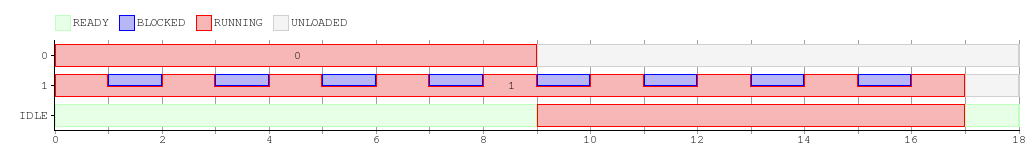
\includegraphics[scale=0.5]{graficos/inherente.png}
  \caption{Procesamiento simultáneo de una tarea I/O y otra de uso\_CPU}
\end{figure}

En el caso mostrado en el gráfico de arriba, ambas tareas requieren de 10 ticks de cpu para finalizar. Sin embargo, la tarea bloqueante tarda el doble de tiempo en terminar. 

En el ejercicio 5 implementamos un scheduler en base al paper ''Lottery scheduling''. El mismo está diseñado para equilibrar esta desigualdad entre el \emph{turn-around} de las tareas relacionado con el
naturaleza de las mismas. El scheduler seleccionea la tarea a la cual será asignado el procesador durante el próximo quantum mediante un sorteo, en donde las probabilidades de ganar
de cada una son inversamente proporcionales a la fracción de quantum que utilizaron la última vez que fueron ganadoras. Para ello se utiliza un sistema de \textbf{tickets}.
Las tareas que consumieron la totalidad del quantum disponen de un único ticket, mientras que las tareas que consumieron una fracción $\frac{f}{q}$ del quantum disponen de $\frac{q}{f}$ tickets (redondeado
hacia arriba). La tarea a la cual se le asignará el procesador durante el próximo quantum será la que tenga el ticket ganador del sorteo entre la totalidad de los mismos.

De esta manera, las tareas de I/O tendrán más probabilidades de ganar los sorteos respecto a aquellas que utilizan la totalidad del CPU. Esto provoca una reducción en el \emph{waiting time} de las mismas 
(ya que deben esperar menos para volver a correr), y por lo tanto también en su \emph{turn-around} time.

\subsubsection{Estructuras auxiliares}

\begin{itemize}
  \item vector<int> cpu\_quantum: Arreglo en donde hay una posición por cada uno de los cores. En cada una queda registro de la cantidad de ticks durante los cuales el procesador ha permanecido
  en posesión del proceso actual. 
  \item semilla: parámetro inicial que determina el inicio de la secuencia pseudoaleatoria.
  \item cantTickets: La cantidad de tickets total que participarán en el próximo sorteo.
  \item max\_quantum: Determina la duración del quantum. Sea \emph{core} uno de los procesadores.\\ 
  Cuando cpu\_quantum[core] $\geq$ max\_quantum, la tarea ha consumido la totalidad del quantum y es necesario realizar
  un sorteo para determinar la próxima tarea que será ejecutada.
  \item vector<tarea,\#tickets> tareasReady: Arreglo que contiene las tareas listas para correr, junto con la cantidad de tickets con la que participarán en el sorteo.$\geq$ max\_quantum, la tarea ha consumido la totalidad del quantum y es necesario realizar
  \item vector<tarea,\#tickets> tareasBlocked: Arreglo que contiene las tareas bloqueadas junto con la cantidad de tickets con las que participarán en el sorteo cuando vuelvan al estado Ready
\end{itemize}

\subsubsection{Pseudocódigo}

\begin{algorithmic}
  \Function{load}{int pid}
      \State Agrego a tareasReady la tupla <pid,1>
      \State $cantTickets \gets cantTickets+1$;
  \EndFunction
\end{algorithmic}

~

Al ser cargadas, las tareas comienzan inicialmente con un único ticket. Es importante actualizar la variable \emph{cantTickets} para dejar actualizado el sorteo.

~

\begin{algorithmic}
  \Function{unblock}{int pid}
      \State Agrego a tareasReady la tupla <pid,\#tickets>, (\#tickets está almacenado en tareasBlocked).
      \State Elimino de tareasBlocked la tupla <pid,\#tickets>
      \State $cantTickets \gets cantTickets+\#tickets$;
  \EndFunction
\end{algorithmic}

~

Las tareas recientemente desbloqueadas participarán del próximo sorteo, por lo que son agregadas a \emph{tareasReady} y retiradas de \emph{tareasBlocked}.
Es importante actualizar la variable \emph{cantTickets} para dejar actualizado el sorteo.

~

\begin{algorithmic}
  \Function{tick}{int cpu, Motivo m}
      \State $actual \gets$ tarea que está siendo ejecutada por el \emph{cpu} actualmente
      \State $proximo \gets$ actual
      
      \If{m==EXIT}
	  \State cpu\_quantum[cpu]=0 (Reseteo el quantum)
	  \If{!tareasReady.empty()}
	      \State $proximo \gets lottery()$
	  \Else
	      \State $proximo \gets IDLE\_TASK$
	  \EndIf
      \EndIf
      \State
      \If{m==BLOCK}
	  \State cpu\_quantum[cpu]++ 
	  \State \#tickets = $\frac{max\_quantum}{cpu\_quantum[cpu]}$ 
	  \State
	  \State (La tarea se bloqueó, por lo que no utilizó la totalidad del quantum.
	  \State Se le asigna una cantidad de tickets inversamente proporcional 
	  \State a la fracción de quantum que haya utilizado.)
	  \State
	  \State Agrego a tareasBlocked la tupla <actual,\#tickets>
	  \State cpu\_quantum[cpu] $\gets 0$
	  \If{!tareasReady.empty()}
	      \State $proximo \gets lottery()$
	  \Else
	      \State $proximo \gets IDLE\_TASK$
	  \EndIf
      \EndIf
      \State
      \If{m==TICK}
	  \State cpu\_quantum[cpu]++
	  \If{actual==IDLE\_TASK}
	      \If{!tareasReady.empty()}
		  \State cpu\_quantum[cpu]=0 
		  \State $proximo \gets lottery()$
	      \EndIf
	      \State(Si no hay otras tareas, continúo ejecutando la IDLE)
	  \Else(se está ejecutando una tarea)
	      \If{cpu\_quantum $\geq$ max\_quantum}
		  \If{!tareasReady.empty()}
		      \State cpu\_quantum[cpu]=0 (Reseteo el quantum)
		      \State $proximo \gets lottery()$
		  \EndIf
		  \State(Si no hay otras tareas, continúo ejecutando la misma)
	      \EndIf
	   \EndIf
      \EndIf
  \EndFunction
\end{algorithmic}

~

\begin{algorithmic}
  \Function{lottery}{}
	\State $suma \gets 0$
      	\State $semilla++$
	\State srand(semilla)
	\State $ticketGanador \gets (rand() \% cantTickets)+1$
	\For{$i \gets 0$ to tareasReady.size()}
		\State $suma \gets suma+ \#tickets$ de tarea i		
		\If{$ticketGanador \leq suma$}
			\State $res \gets$ tarea i
			\State $cantTickets \gets $ \#tickets de tarea i	
			\State Borro la tarea i de tareasReady
			\State break
		\EndIf
	\EndFor	
	\State \Return res
  \EndFunction
\end{algorithmic}

~

Para realizar el sorteo se selecciona un número aleatiro utilizando las funciones rand y srand (ya explicadas con anterioridad).

Incrementamos el valor de la semilla para que la próxima vez el sorteo se realice con una secuencia pseudoaleatoria distinta.

El sorteo se realiza específicamente en la línea: $ticketGanador$ = ( rand() \% (cantTickets) ) + 1.

Recorremos la lista hasta encontrar la tarea con el ticket ganador.

Decrementamos la cantidad de tickets y retiramos $res$ de la lista de tareasReady.

~

\begin{figure}[H]
  \centering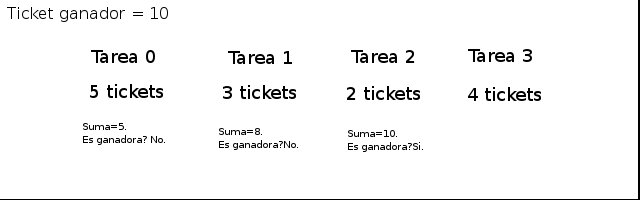
\includegraphics[scale=0.5]{graficos/lottery.jpg}
  \caption{Funcionamiento de lottery()}
\end{figure}

~

\subsubsection{Experimentando con SchedLottery con compensation tickets}

Simulemos en primer lugar el comportamiento de nuestro scheduler para un lote de tareas de cálculo: es decir, procesos que no 
efectúan instrucciones de I/0. A lo largo de la ejecución habrá tantos tickets como tareas, cada uno correspondiente a una
tarea distinta. Por lo tanto, dado un lote de $n$ tareas cada una tiene una probabilidad de $\frac{1}{n}$ de obtener el procesador
en el próximo quantum. El comportamiento esperado es de alguna forma similar al de round robin, ya que se espera que cada $n$
quantums, cada tarea haya sido ejecutada durante 1 quantum.


\begin{figure}[H]
  \centering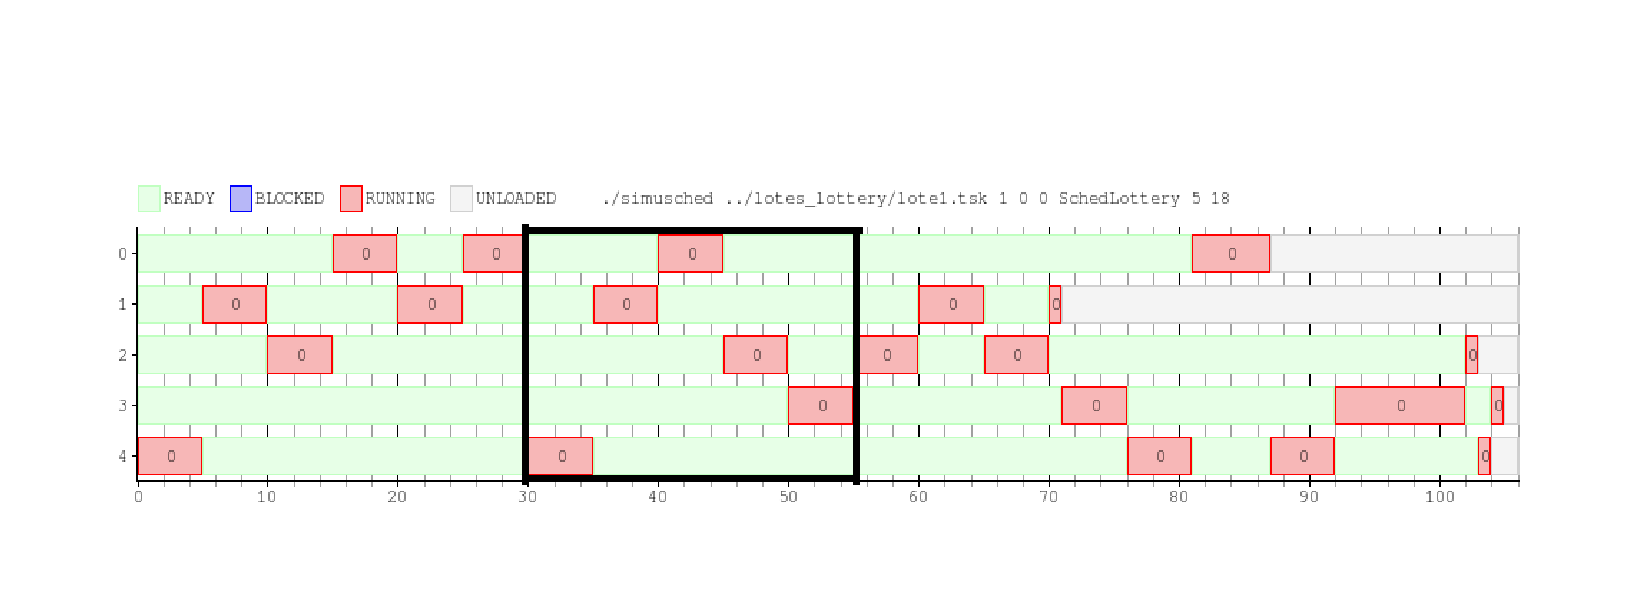
\includegraphics[scale=0.5]{graficos/lottery_cpu.pdf}
  \caption{SchedLottery en un lote de procesamiento cientifico. lote: *5 TaskCPU 20.
	1 core, cambio de contexto y migración = 0, quantum = 5}
\end{figure}

~

Efectivamente, en el recuadro negro que aparece en la figura el comportamiento es muy similar al de Round-Robin.

\begin{itemize}
	\item tarea 0: wt:16.5, ta:87
	\item tarea 1: wt:10, ta:71
	\item tarea 2: wt:16.4, ta:103
	\item tarea 3: wt:21, ta:105
	\item tarea 4: wt:20.75, ta:104
	\item  Waiting time: 16.93
	\item  Turnaround time: 94
\end{itemize} 

Observemos que tanto el wating time como el turn around time de cada una de las tareas no difiere demasiado entre sí (tal como hubiera sucedido en el Round-Robin).
Si realizamos 40 corridas del mismo experimento, para un único core pero variando el quantum entre 1 y 5, obtenemos los siguientes gráficos, en donde se muestran
el waiting-time promedio y el $turn-around$ promedio.


\FloatBarrier

\begin{figure}
\hfill
\subfigure[]{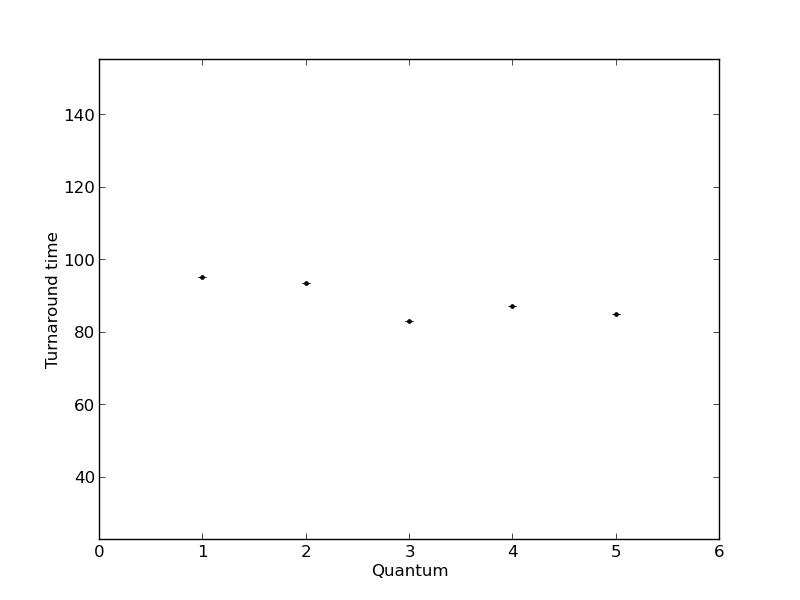
\includegraphics[width=8.75cm]{graficos/lottery_cpu_ta.jpg}}
\hfill
\subfigure[]{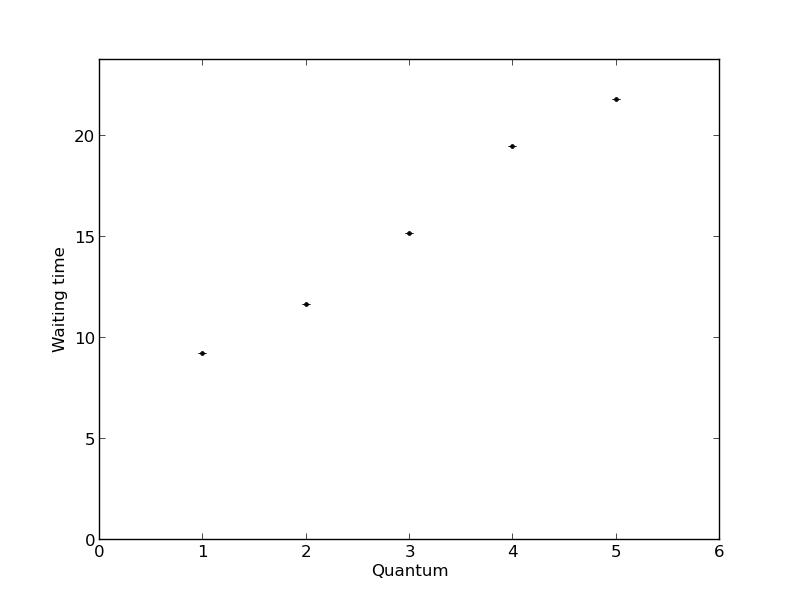
\includegraphics[width=8.75cm]{graficos/lottery_cpu_wt.jpg}}
\hfill
\caption{Turn around time y waiting time del SchedLottery del mismo lote de procesamiento cientìfico con los mismos paràmetros,
	pero variando los quantums entre 1 y 5}
\end{figure}

El waiing-time promedio de 40 repeticiones para 5 cores es de 17.5, cercano al experimento particular aislado, en donde obtuvimos 16.93.
El turn-time promedio de 40 repeticiones para 5 cores es de 85, cercano al experimento particular aislado, en donde obtuvimos 94.

~

Si comparamos los resultados obtenidos con los de un scheduler round-robin obtenemos:

\begin{figure}
\hfill
\subfigure[]{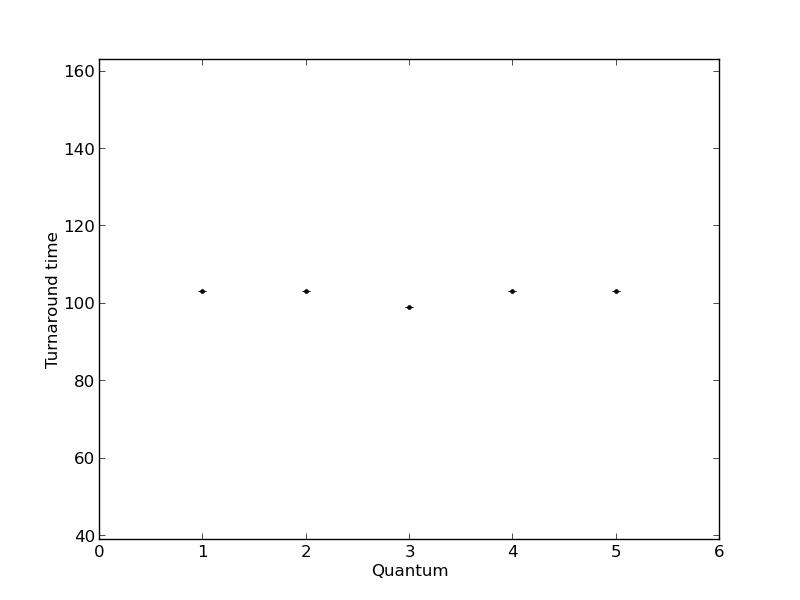
\includegraphics[width=8.75cm]{graficos/lottery_rr_ta.jpg}}
\hfill
\subfigure[]{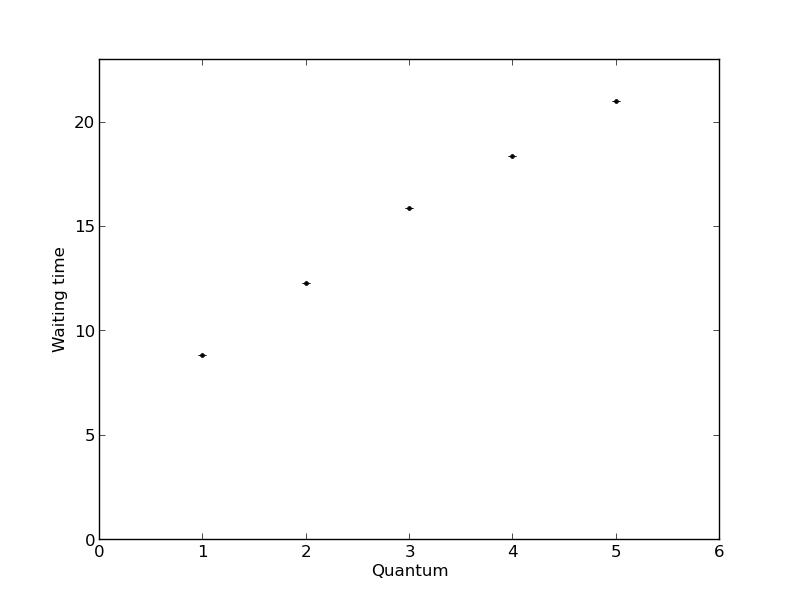
\includegraphics[width=8.75cm]{graficos/lottery_rr_wt.jpg}}
\hfill
\caption{Turn around time y waiting time del Round Robin del mismo lote de procesamiento cientìfico con los mismos paràmetros,
	pero variando los quantums entre 1 y 5}
\end{figure}

Tal como era esperable, para lotes con tareas de igual cantidad de tickets ambos schedulers se comportan de forma muy similar.

\FloatBarrier


En el ejercicio 5 implementamos un scheduler en base al paper ''Lottery scheduling''. El mismo está diseñado para equilibrar esta desigualdad entre el \emph{turn-around} de las tareas relacionado con el
Para ejemplificar lo mencionado anteriormente, supongamos que en una computadora de un solo core se han lanzado dos procesos que corren en simultáneo. El primero de ellos, al cual llamaremos $A$, utiliza
activamente el CPU sin necesidad de hacer llamados al sistema o esperar que se liberen recursos de la máquina (podría ser, por ejemplo, el caso de una aplicación científica que ejecuta gran cantidad de 
cuentas). Por otro lado tenemos a la tarea $B$, que ejecuta una instrucción bloqueante cada cierto tiempo, desbloquéandose luego de una cierta cantidad de ticks del reloj. Supongamos también que ambos conviven
con otros procesos que también están siendo ejecutados por el cpu. En el caso de un scheduler Round Robin, a lo largo de una ronda se le asigna un quantum a cada proceso. Sin embargo, notemos que mientras
la tarea $A$ utiliza la totalidad del quantum que le han asignado, $B$ usa únicamente una fracción: $\frac{f}{q}$. De esta manera, luego de sucesivas rondas la tarea $A$ ha sido ejecutada un tiempo
considerablemente mayor al de $B$.

Para solucionar este problema, la idea es que el scheduler seleccione la próxima a ser ejecutada mediante el sorteo de una lotería, en donde aquellas tareas que utilicen solamente una fracción del quantum
tengan más probabilidades de ser las ganadoras. Para lograr este objetivo, utilizamos un sistema de ''compensation tickets'', que funciona de la siguiente manera:

- Las tareas que llegan por primera vez entran con una cantidad equivalente a $\frac{\#tickss}{quantum}$. Por ejemplo, si cada quantum consta de 8 ticks, entonces cada
proceso recibirá 8 tickets iniciales, con lo cual evitamos que las tareas recién ingresadas sufran de inanición (se les dé la oportunidad de correr para conocer su tipo, 
y comepensarlos (o no) con la cantidad de tickets correspondiente).

- Cuando una tarea es desalojada debido a una llamada bloqueante, lo más probable es que solamente haya utilizado una fracción del quantum. Sea esta última $\frac{f}{q}$,
en donde q es igual a $\frac{\#tickss}{quantum}$ y f la cantidad de ticks consumidos por la tarea durante el último llamado.
Anteriormente habíamos dicho que el scheduler debía encargarse de que todas las tareas corrieran una cantidad de tiempo lo más similar posible a las demás, y que para ello utilizaba
el sistema de compensation tickets. Nuestro mecanismo hace que la tarea ingrese a la cola de Ready's con $\frac{q}{f}$ tickets, con lo cual tiene una probabilidad de ganar
inversamente proporcional a la fracción de quantum que está usando.

- Cuando se produce un tick y el scheduler detecta que la tarea consumió la totalidad de su quantum, la misma es desalojada y encolada en el vector de Ready's con un solo ticket.

~


Poniendo en un ejemplo lo anteriormente mencionado, supongamos una máquina con un scheduler con
un quantum de 8 ticks manejando temporalmente 
1 tarea bloqueante $A$ (cuyos bloqueos duran 1 ciclo), y 2 tareas $B$ y $C$ que consumen CPU. En un principio todas entran al sorteo con 8
tickets. Sin embargo, luego de que las tres han corrido por lo menos una vez, siempre entrarán al sorteo con una misma cantidad: $A=8, \ B=1, \ C=1$, con un total de
10 tickets en circulación. Con estos valores, se espera que cada 10 sorteos (número que coincide con la cantidad de tickets en circulación): 8 sean ganados por A,
1 sea ganado por B y 1 por C, con lo cual todas estarían corriendo la misma cantidad de ticks en el cpu. 




 
